\documentclass[12pt, a4paper]{article}

% --- STANDARD PACKAGES ---
\usepackage[margin=1in]{geometry} % Set margins
\usepackage{amsmath, amssymb, amsthm} % AMS math packages
\usepackage{graphicx} % For including figures
\usepackage[font=small, labelfont=bf]{caption} % Customize captions
\usepackage{booktabs} % For professional-looking tables
\usepackage{hyperref} % For hyperlinks (optional, but good)
\hypersetup{colorlinks=true, linkcolor=blue, citecolor=blue, urlcolor=blue}

% --- THEOREM ENVIRONMENTS ---
\theoremstyle{definition}
\newtheorem{definition}{Definition}[section]
\newtheorem{example}{Example}[section] % Standard example environment
\newtheorem{remark}{Remark}[section]

\theoremstyle{plain}
\newtheorem{theorem}{Theorem}[section]
\newtheorem{corollary}{Corollary}[section]
\newtheorem{lemma}{Lemma}[section]
% Custom proof environment start text
\renewcommand{\proofname}{\bfseries Proof}

% --- CUSTOM MATH COMMANDS ---
\newcommand{\Prob}[1]{\mathbb{P}\left[#1\right]} % Probability P[ ]
\newcommand{\condProb}[2]{\mathbb{P}\left[#1 \mid #2\right]} % Conditional Prob P[ | ]
\newcommand{\intersect}{\cap} % Intersection
\newcommand{\union}{\cup}     % Union
\newcommand{\reals}{\mathbb{R}}     % Real numbers
\newcommand{\samplespace}{\Omega} % Sample space Omega
\newcommand{\comp}[1]{#1^c} % Complement (superscript c)
\newcommand{\emptySet}{\emptyset} % Empty set

\usepackage{setspace}

% Use the biblatex package
\usepackage[backend=biber, style=numeric, sorting=none]{biblatex}

% Link your .bib file
\addbibresource{references.bib}

% --- DOCUMENT START ---
\begin{document}

\onehalfspacing % Apply 1.5 spacing to the whole document

\title{Set Theory and Probability II}
\author{Mahbubur Rahman Khan}
\date{October 26, 2025}
\maketitle

\begin{abstract}
    This document covers foundational concepts in probability theory. Key topics discussed include conditional probability (definition, properties, multiplication rule), statistical independence (definitions via product rule and conditional probability, properties, distinction from disjoint events, independence of multiple events), the law of total probability, and Bayes' theorem (including its proof and the full formula incorporating total probability). This material is synthesized from faculty-provided resources (\cite{FacultyNotes}) and standard probability textbooks by Sheldon M. Ross (\cite{Ross}) and Stanley H. Chan (\cite{Chan}).
\end{abstract}

\tableofcontents
\newpage

\section{Applications of Total Probability and Bayes' Theorem}

Two fundamental principles frequently applied in probability are the \textbf{Law of Total Probability}, which facilitates calculating the probability of an event by partitioning the sample space, and \textbf{Bayes' Theorem}, which enables the calculation of posterior probabilities by "inverting" conditional probabilities.

\begin{example}[Tennis Tournament / Player Types \cite{FacultyNotes, Chan}]
\textbf{(Example)} Consider a tennis tournament with three categories of players: A, B, and C.
\begin{itemize}
    \item \textbf{Prior Probabilities (Partition):} The distribution of player types is:
        \begin{itemize}
            \item $\Prob{A} = 0.5$
            \item $\Prob{B} = 0.25$
            \item $\Prob{C} = 0.25$
        \end{itemize}
        These form a partition as $A, B, C$ are disjoint and $\Prob{A}+\Prob{B}+\Prob{C} = 1$.
    \item \textbf{Conditional Probabilities (Win Rates):} Let $W$ denote the event that you win a match. Your probability of winning depends on the opponent's type:
        \begin{itemize}
            \item $\condProb{W}{A} = 0.3$
            \item $\condProb{W}{B} = 0.4$
            \item $\condProb{W}{C} = 0.5$
        \end{itemize}
\end{itemize}
\textbf{Question (a):} Determine the overall probability of winning a randomly selected match, $\Prob{W}$.\\
Applying the \textbf{Law of Total Probability}, we sum the win probabilities over the partition \{A, B, C\}:
\begin{itemize}
    \item \textbf{Formula:} $\Prob{W} = \condProb{W}{A}\Prob{A} + \condProb{W}{B}\Prob{B} + \condProb{W}{C}\Prob{C}$ \cite{FacultyNotes, Chan}.
    \item \textbf{Calculation:}
        \[ \Prob{W} = (0.3)(0.5) + (0.4)(0.25) + (0.5)(0.25) = 0.15 + 0.10 + 0.125 = 0.375 \]
\end{itemize}
\textbf{Question (b):} Given that you have won a match, what is the probability that your 
opponent was a type A player, $\condProb{A}{W}$?\\
Applying \textbf{Bayes' Theorem}, we calculate the posterior probability:
\begin{itemize}
    \item \textbf{Formula:} $\condProb{A}{W} = \frac{\condProb{W}{A}\Prob{A}}{\Prob{W}}$ \cite{FacultyNotes, Chan}.
    \item \textbf{Calculation:}
        \[ \condProb{A}{W} = \frac{(0.3)(0.5)}{0.375} = \frac{0.15}{0.375} = 0.4 \quad \cite{FacultyNotes, Chan} \]
\end{itemize}
\end{example}

\begin{example}[Laboratory Blood Test (Base Rate Fallacy) \cite{Ross}]
\textbf{(Example)} This example illustrates the importance of base rates in conditional probability calculations.
\begin{itemize}
    \item \textbf{Problem:} A diagnostic test for a specific disease has the following characteristics:
        \begin{itemize}
            \item Sensitivity: The test correctly identifies the disease (positive result) in 95\% of cases where it is present.
            \item False Positive Rate: The test incorrectly indicates the disease (positive result) in 1\% of cases where it is absent \cite{Ross}.
        \end{itemize}
    \item \textbf{Base Rate:} The prevalence of the disease in the population is 0.5\% (or 0.005).
    \item \textbf{Question:} If a randomly selected individual tests positive, what is the probability they actually have the disease?
\end{itemize}
\textbf{Setup:}
\begin{itemize}
    \item Let $D$ be the event that the person has the disease. $\Prob{D} = 0.005$.
    \item Let $\comp{D}$ be the event that the person is healthy. $\Prob{\comp{D}} = 1 - 0.005 = 0.995$.
    \item Let $E$ be the event that the test result is positive.
\end{itemize}
\textbf{Conditional Probabilities:}
\begin{itemize}
    \item $\condProb{E}{D} = 0.95$ (Sensitivity).
    \item $\condProb{E}{\comp{D}} = 0.01$ (False Positive Rate).
\end{itemize}
\textbf{Goal:} Calculate $\condProb{D}{E}$.
\begin{itemize}
    \item \textbf{Step 1: Calculate $\Prob{E}$ using the Law of Total Probability.}
        \[ \Prob{E} = \condProb{E}{D}\Prob{D} + \condProb{E}{\comp{D}}\Prob{\comp{D}} \]
        \[ \Prob{E} = (0.95)(0.005) + (0.01)(0.995) = 0.00475 + 0.00995 = 0.0147 \]
    \item \textbf{Step 2: Apply Bayes' Formula.}
        \[ \condProb{D}{E} = \frac{\condProb{E}{D}\Prob{D}}{\Prob{E}} = \frac{(0.95)(0.005)}{0.0147} \approx 0.323 \]
\end{itemize}
\textbf{Conclusion:} Despite the test's 95\% sensitivity, the probability that a person with a positive test result actually has the disease is only approximately 32.3\%. This highlights the impact of the low base rate of the disease \cite{Ross}.
\end{example}

\begin{example}[Multiple Choice Test \cite{Ross}]
\textbf{(Example)} This example demonstrates Bayesian updating of belief based on evidence.
\begin{itemize}
    \item \textbf{Problem:} A student answers a multiple-choice question with $m$ options \cite{Ross}.
        \begin{itemize}
            \item The probability the student knows the answer is $p$.
            \item The probability the student guesses is $1-p$.
            \item If guessing, the probability of selecting the correct answer is $1/m$.
        \end{itemize}
    \item \textbf{Question:} Given the student answered correctly, what is the probability they knew the answer?
\end{itemize}
\textbf{Setup:}
\begin{itemize}
    \item Let $K$ be the event the student knows the answer. $\Prob{K} = p$.
    \item Let $\comp{K}$ be the event the student guesses. $\Prob{\comp{K}} = 1-p$.
    \item Let $C$ be the event the answer is correct.
\end{itemize}
\textbf{Conditional Probabilities:} $\condProb{C}{K} = 1$ and $\condProb{C}{\comp{K}} = 1/m$.
\textbf{Goal:} Calculate $\condProb{K}{C}$.
\begin{itemize}
    \item \textbf{Step 1: Calculate $\Prob{C}$ using the Law of Total Probability.}
        \[ \Prob{C} = \condProb{C}{K}\Prob{K} + \condProb{C}{\comp{K}}\Prob{\comp{K}} \]
        \[ \Prob{C} = (1)(p) + (1/m)(1-p) \]
    \item \textbf{Step 2: Apply Bayes' Formula.}
        \[ \condProb{K}{C} = \frac{\condProb{C}{K}\Prob{K}}{\Prob{C}} = \frac{p}{p + (1/m)(1-p)} \]
        Simplifying yields: $\condProb{K}{C} = \frac{mp}{1 + (m-1)p}$.
\end{itemize}
For instance, if $m=5$ and $p=0.5$, then $\condProb{K}{C} = \frac{5(0.5)}{1+(4)(0.5)} = \frac{2.5}{3} = 5/6$ \cite{Ross}.
\end{example}

\section{Conditional Probability}

Conditional probability addresses the likelihood of an event occurring given that another event has already occurred. This knowledge often modifies the original probability assessment \cite{Chan, FacultyNotes}. In many situations, we do not know the precise outcome of an experiment, but we have partial information suggesting that the outcome belongs to a specific event (subset of the sample space). Conditional probability formalizes reasoning under such partial information \cite{FacultyNotes}.

\begin{example}[Intuitive Example \cite{Ross}]
\textbf{(Example)} Consider the experiment of tossing two fair dice.
\begin{itemize}
    \item The probability that the sum is 6 is $\Prob{\text{Sum}=6} = 5/36$. The sample space consists of 36 equally likely outcomes. The event includes $\{(1,5), (2,4), (3,3), (4,2), (5,1)\}$.
    \item Suppose it is known that the first die resulted in a 4 \cite{Ross}.
    \item This information reduces the effective sample space to 6 outcomes: \\ $\{(4,1), (4,2), (4,3), (4,4), (4,5), (4,6)\}$ \cite{Ross}.
    \item Assuming these outcomes remain equally likely within the reduced space, each now has a probability of $1/6$ \cite{Ross}.
    \item Within this reduced sample space, only the outcome $(4,2)$ results in a sum of 6.
    \item Thus, the \textit{conditional probability} that the sum is 6, \textit{given} the first die was 4, is $1/6$.
\end{itemize}
\end{example}

\subsection{Formal Definition}

The intuition involves considering the conditioning event F as the new (reduced) sample space. For event E to also occur under this condition, the outcome must lie within the intersection $E \intersect F$. The probability is then normalized by the probability of this new sample space, $\Prob{F}$ \cite{Ross, Chan, FacultyNotes}.

\begin{definition}[Conditional Probability \cite{Ross, Chan, FacultyNotes}]
\textbf{(Definition)} Given a probability space $(\samplespace, \mathcal{F}, \Prob{\cdot})$, the \textbf{conditional probability} of event E given that event F has occurred (assuming $\Prob{F} > 0$) is defined as:
\[ \condProb{E}{F} \stackrel{\text{def}}{=} \frac{\Prob{E \intersect F}}{\Prob{F}} \]
\end{definition}

\begin{figure}[ht]
    \centering
    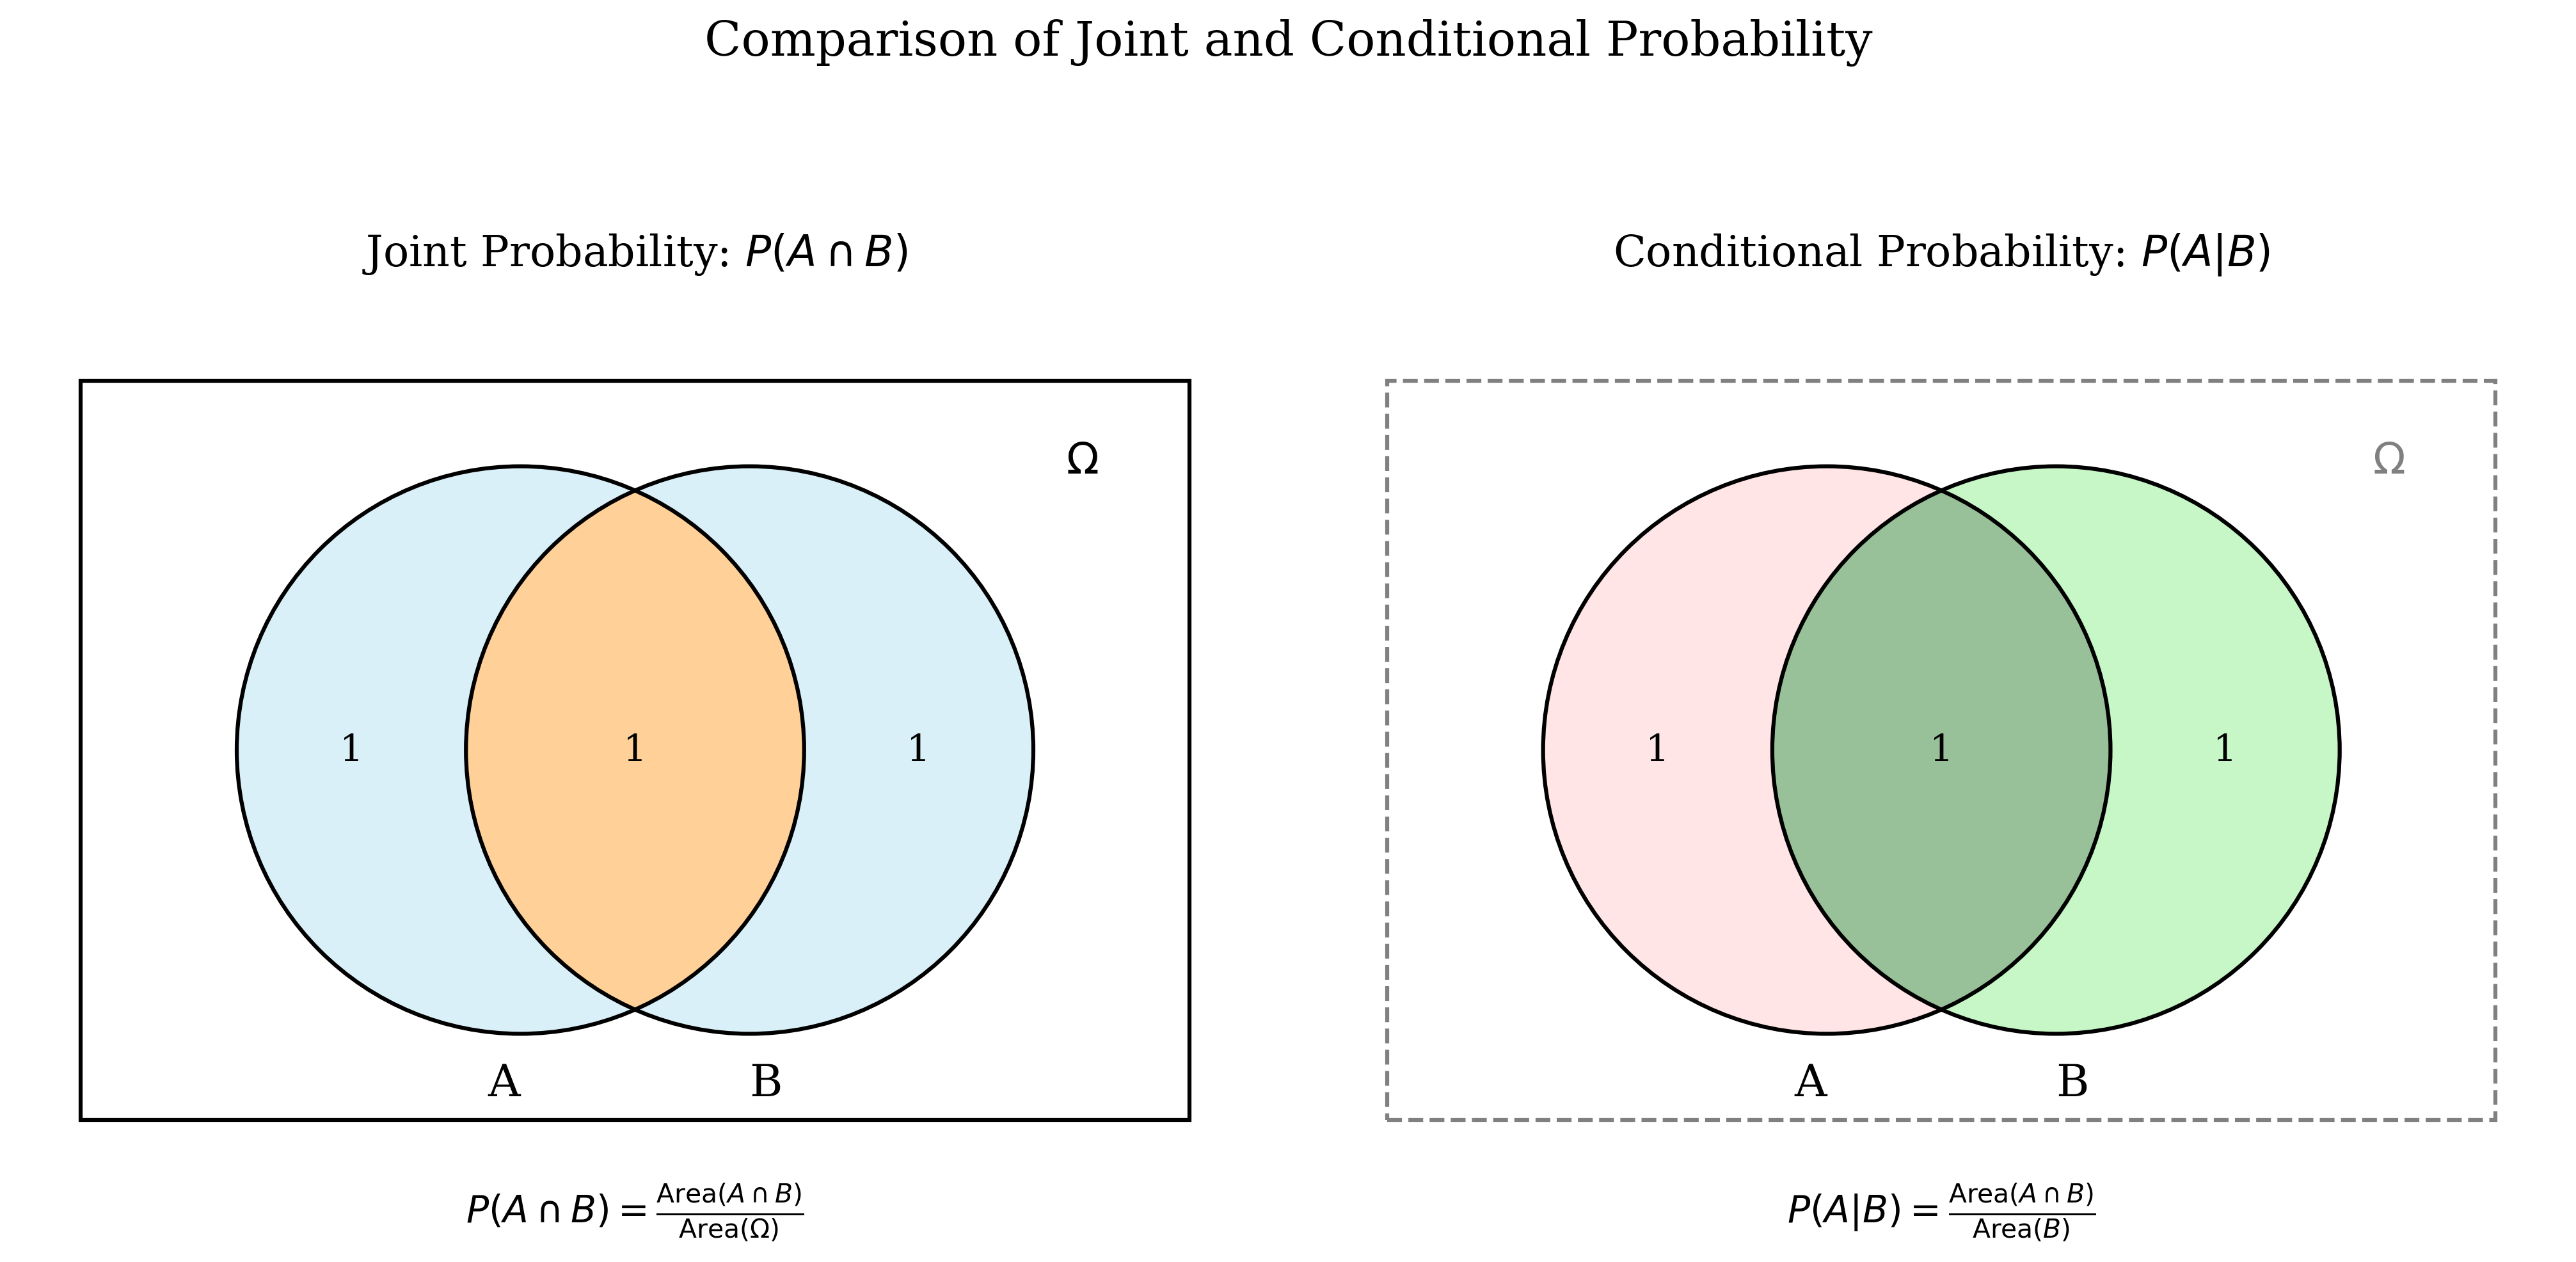
\includegraphics[width=0.9\textwidth]{figure_1.png}
    \caption{Comparison of joint probability $\Prob{A \intersect B}$ and conditional probability $\condProb{A}{B}$ \cite{Chan}.}
    \label{fig:condprob_vis}
\end{figure}

\subsection{The Multiplication Rule}

Rearranging the definition provides the \textbf{multiplication rule}:
\[ \Prob{E \intersect F} = \Prob{F}\condProb{E}{F} \quad (\text{if } \Prob{F} > 0) \]
This rule is fundamental for calculating the probability of the simultaneous occurrence of events, particularly in sequential experiments \cite{FacultyNotes}.

\begin{example}[Drawing from an Urn \cite{Ross}]
\textbf{(Example)}
\begin{itemize}
    \item \textbf{Problem:} An urn contains 7 black and 5 white balls. Two balls are drawn sequentially \textit{without replacement}. Calculate the probability that both drawn balls are black \cite{Ross}.
    \item Let $F$ be the event that the first ball drawn is black.
    \item Let $E$ be the event that the second ball drawn is black.
    \item We seek $\Prob{E \intersect F}$.
    \item The probability of the first ball being black is $\Prob{F} = 7/12$.
    \item Given the first was black, there are 6 black and 5 white balls remaining (11 total). Thus, the conditional probability of the second being black given the first was black is $\condProb{E}{F} = 6/11$ \cite{Ross}.
    \item Applying the multiplication rule: $\Prob{E \intersect F} = \Prob{F}\condProb{E}{F} = \left(\frac{7}{12}\right)\left(\frac{6}{11}\right) = \frac{42}{132}$.
\end{itemize}
\end{example}

\subsection{Examples of Calculating Conditional Probability}

\begin{example}[Die Roll \cite{Chan, FacultyNotes}]
\textbf{(Example)}
\begin{itemize}
    \item Experiment: Roll a fair six-sided die. Let $A = \{\text{outcome is 3}\}$ and $B = \{\text{outcome is odd}\}$ \cite{Chan}.
    \item Calculate $\condProb{A}{B}$ and $\condProb{B}{A}$.
\end{itemize}
\textbf{Probabilities:}
\begin{itemize}
    \item $\Prob{A} = \Prob{\{3\}} = 1/6$.
    \item $\Prob{B} = \Prob{\{1, 3, 5\}} = 3/6 = 1/2$.
    \item $A \intersect B = \{3\}$. $\Prob{A \intersect B} = 1/6$.
\end{itemize}
\textbf{Calculations:}
\begin{itemize}
    \item $\condProb{A}{B} = \frac{\Prob{A \intersect B}}{\Prob{B}} = \frac{1/6}{3/6} = 1/3$. Interpretation: Given the outcome is odd, the reduced sample space is $\{1, 3, 5\}$, making the probability of getting a 3 equal to 1/3 \cite{Chan}.
    \item $\condProb{B}{A} = \frac{\Prob{A \intersect B}}{\Prob{A}} = \frac{1/6}{1/6} = 1$. Interpretation: Given the outcome is 3, it is certain (probability 1) that the outcome is odd \cite{Chan}.
\end{itemize}
\end{example}

\begin{example}[Tetrahedral Die \cite{Chan}]
\textbf{(Example)}
\begin{itemize}
    \item Experiment: Roll a fair 4-sided die twice. Let $X$ be the result of the first roll and $Y$ the result of the second. The sample space has $4 \times 4 = 16$ equally likely outcomes.
    \item Define events: $B = \{\min(X, Y) = 2\}$ and $M = \{\max(X, Y) = 3\}$.
    \item \textbf{Question:} Calculate $\condProb{M}{B}$.
\end{itemize}
\begin{figure}[ht]
    \centering
    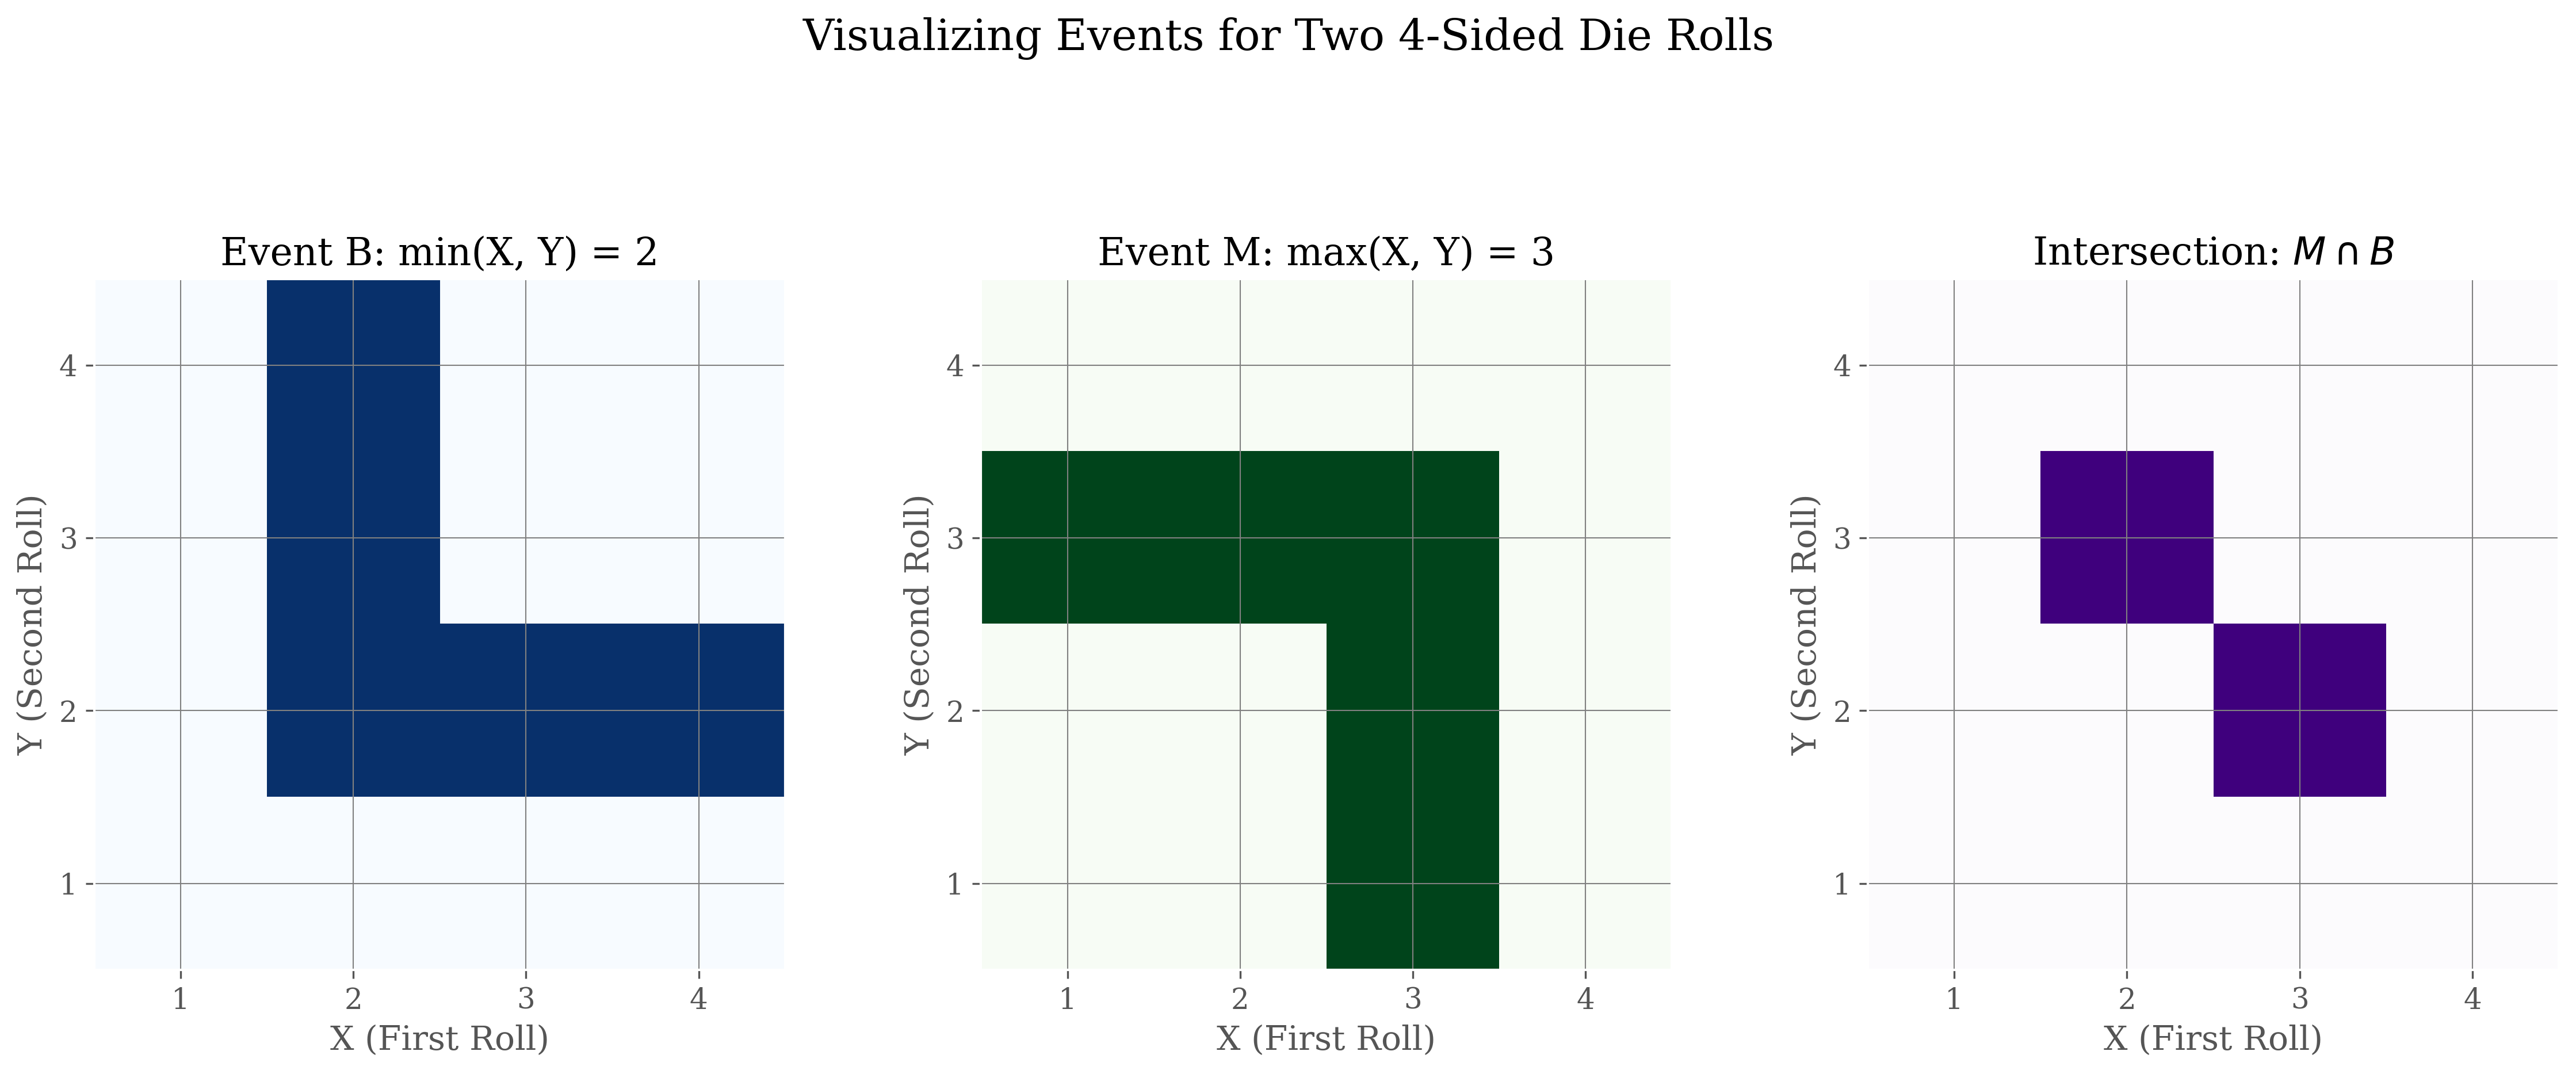
\includegraphics[width=0.9\textwidth]{figure_2.png}
    \caption{Visualization of events B, M, and their intersection for the 4-sided die example \cite{Chan}.}
    \label{fig:tetra_die}
\end{figure}
\textbf{Probabilities:}
\begin{itemize}
    \item Event B consists of 5 outcomes: $\Prob{B} = 5/16$.
    \item Event $M \intersect B$ consists of 2 outcomes: $\Prob{M \intersect B} = 2/16$.
\end{itemize}
\textbf{Calculation:}
\[ \condProb{M}{B} = \frac{\Prob{M \intersect B}}{\Prob{B}} = \frac{2/16}{5/16} = 2/5 \quad \cite{Chan} \]
\end{example}

\subsection{Conditional Probability as a Probability Measure}
For a fixed event B with $\Prob{B}>0$, the function $\condProb{\cdot}{B}$ mapping events A to $\condProb{A}{B}$ satisfies the three axioms of probability \cite{FacultyNotes, Chan}.
\begin{enumerate}
    \item \textbf{Axiom I (Non-negativity):} $\condProb{A}{B} \ge 0$ \cite{FacultyNotes, Chan}.
    \item \textbf{Axiom II (Normalization):} $\condProb{\samplespace}{B} = 1$ \cite{FacultyNotes, Chan}.
    \item \textbf{Axiom III (Additivity):} If A and C are disjoint events, then $\condProb{A \union C}{B} = \condProb{A}{B} + \condProb{C}{B}$ \cite{FacultyNotes, Chan}.
\end{enumerate}
\begin{proof}
\textbf{(Proof)} The proofs follow directly from the definition of conditional probability and the axioms satisfied by the original probability measure $\Prob{\cdot}$ \cite{FacultyNotes, Chan}.
\begin{enumerate}
    \item Non-negativity: Since $\Prob{A \intersect B} \ge 0$ and $\Prob{B} > 0$, the ratio $\condProb{A}{B} = \frac{\Prob{A \intersect B}}{\Prob{B}}$ must be non-negative.
    \item Normalization: $\condProb{\samplespace}{B} = \frac{\Prob{\samplespace \intersect B}}{\Prob{B}} = \frac{\Prob{B}}{\Prob{B}} = 1$.
    \item Additivity:
    \begin{align*}
        \condProb{A \union C}{B} &= \frac{\Prob{(A \union C) \intersect B}}{\Prob{B}} \quad \text{(by def.)} \\
        &= \frac{\Prob{(A \intersect B) \union (C \intersect B)}}{\Prob{B}} \quad \text{(Distributive Law)} \\
        \intertext{Since A and C are disjoint, $(A \intersect B)$ and $(C \intersect B)$ are also disjoint \cite{FacultyNotes, Chan}.}
        &= \frac{\Prob{A \intersect B} + \Prob{C \intersect B}}{\Prob{B}} \quad \text{(Axiom III for P)} \\
        &= \frac{\Prob{A \intersect B}}{\Prob{B}} + \frac{\Prob{C \intersect B}}{\Prob{B}} \\
        &= \condProb{A}{B} + \condProb{C}{B}
    \end{align*}
\end{enumerate}
\end{proof}

\section{Statistical Independence}

\subsection{Definitions}
Statistical independence captures the notion that the occurrence (or non-occurrence) of one event provides no probabilistic information about another event.

\begin{definition}[Independence - Product Rule \cite{FacultyNotes, Chan, Ross}]
\textbf{(Definition)} Events E and F are \textbf{statistically independent} if and only if:
\[ \Prob{E \intersect F} = \Prob{E}\Prob{F} \]
\end{definition}

\begin{definition}[Independence - Conditional Rule \cite{Chan, Ross}]
\textbf{(Definition)} Events E and F (with $\Prob{F}>0$) are independent if and only if:
\[ \condProb{E}{F} = \Prob{E} \]
Equivalently, if $\Prob{E}>0$, independence holds if $\condProb{F}{E} = \Prob{F}$ \cite{Chan, Ross}. This means knowledge that F has occurred does not affect the probability that E occurs \cite{Ross}.
\end{definition}

\begin{remark}
\textbf{(Remark)} The two definitions are equivalent. If $\condProb{E}{F} = \Prob{E}$, substituting into the definition of conditional probability yields $\frac{\Prob{E \intersect F}}{\Prob{F}} = \Prob{E}$, which directly implies $\Prob{E \intersect F} = \Prob{E}\Prob{F}$ (assuming $\Prob{F}>0$) \cite{Chan, FacultyNotes}.
\end{remark}

\begin{figure}[ht]
    \centering
    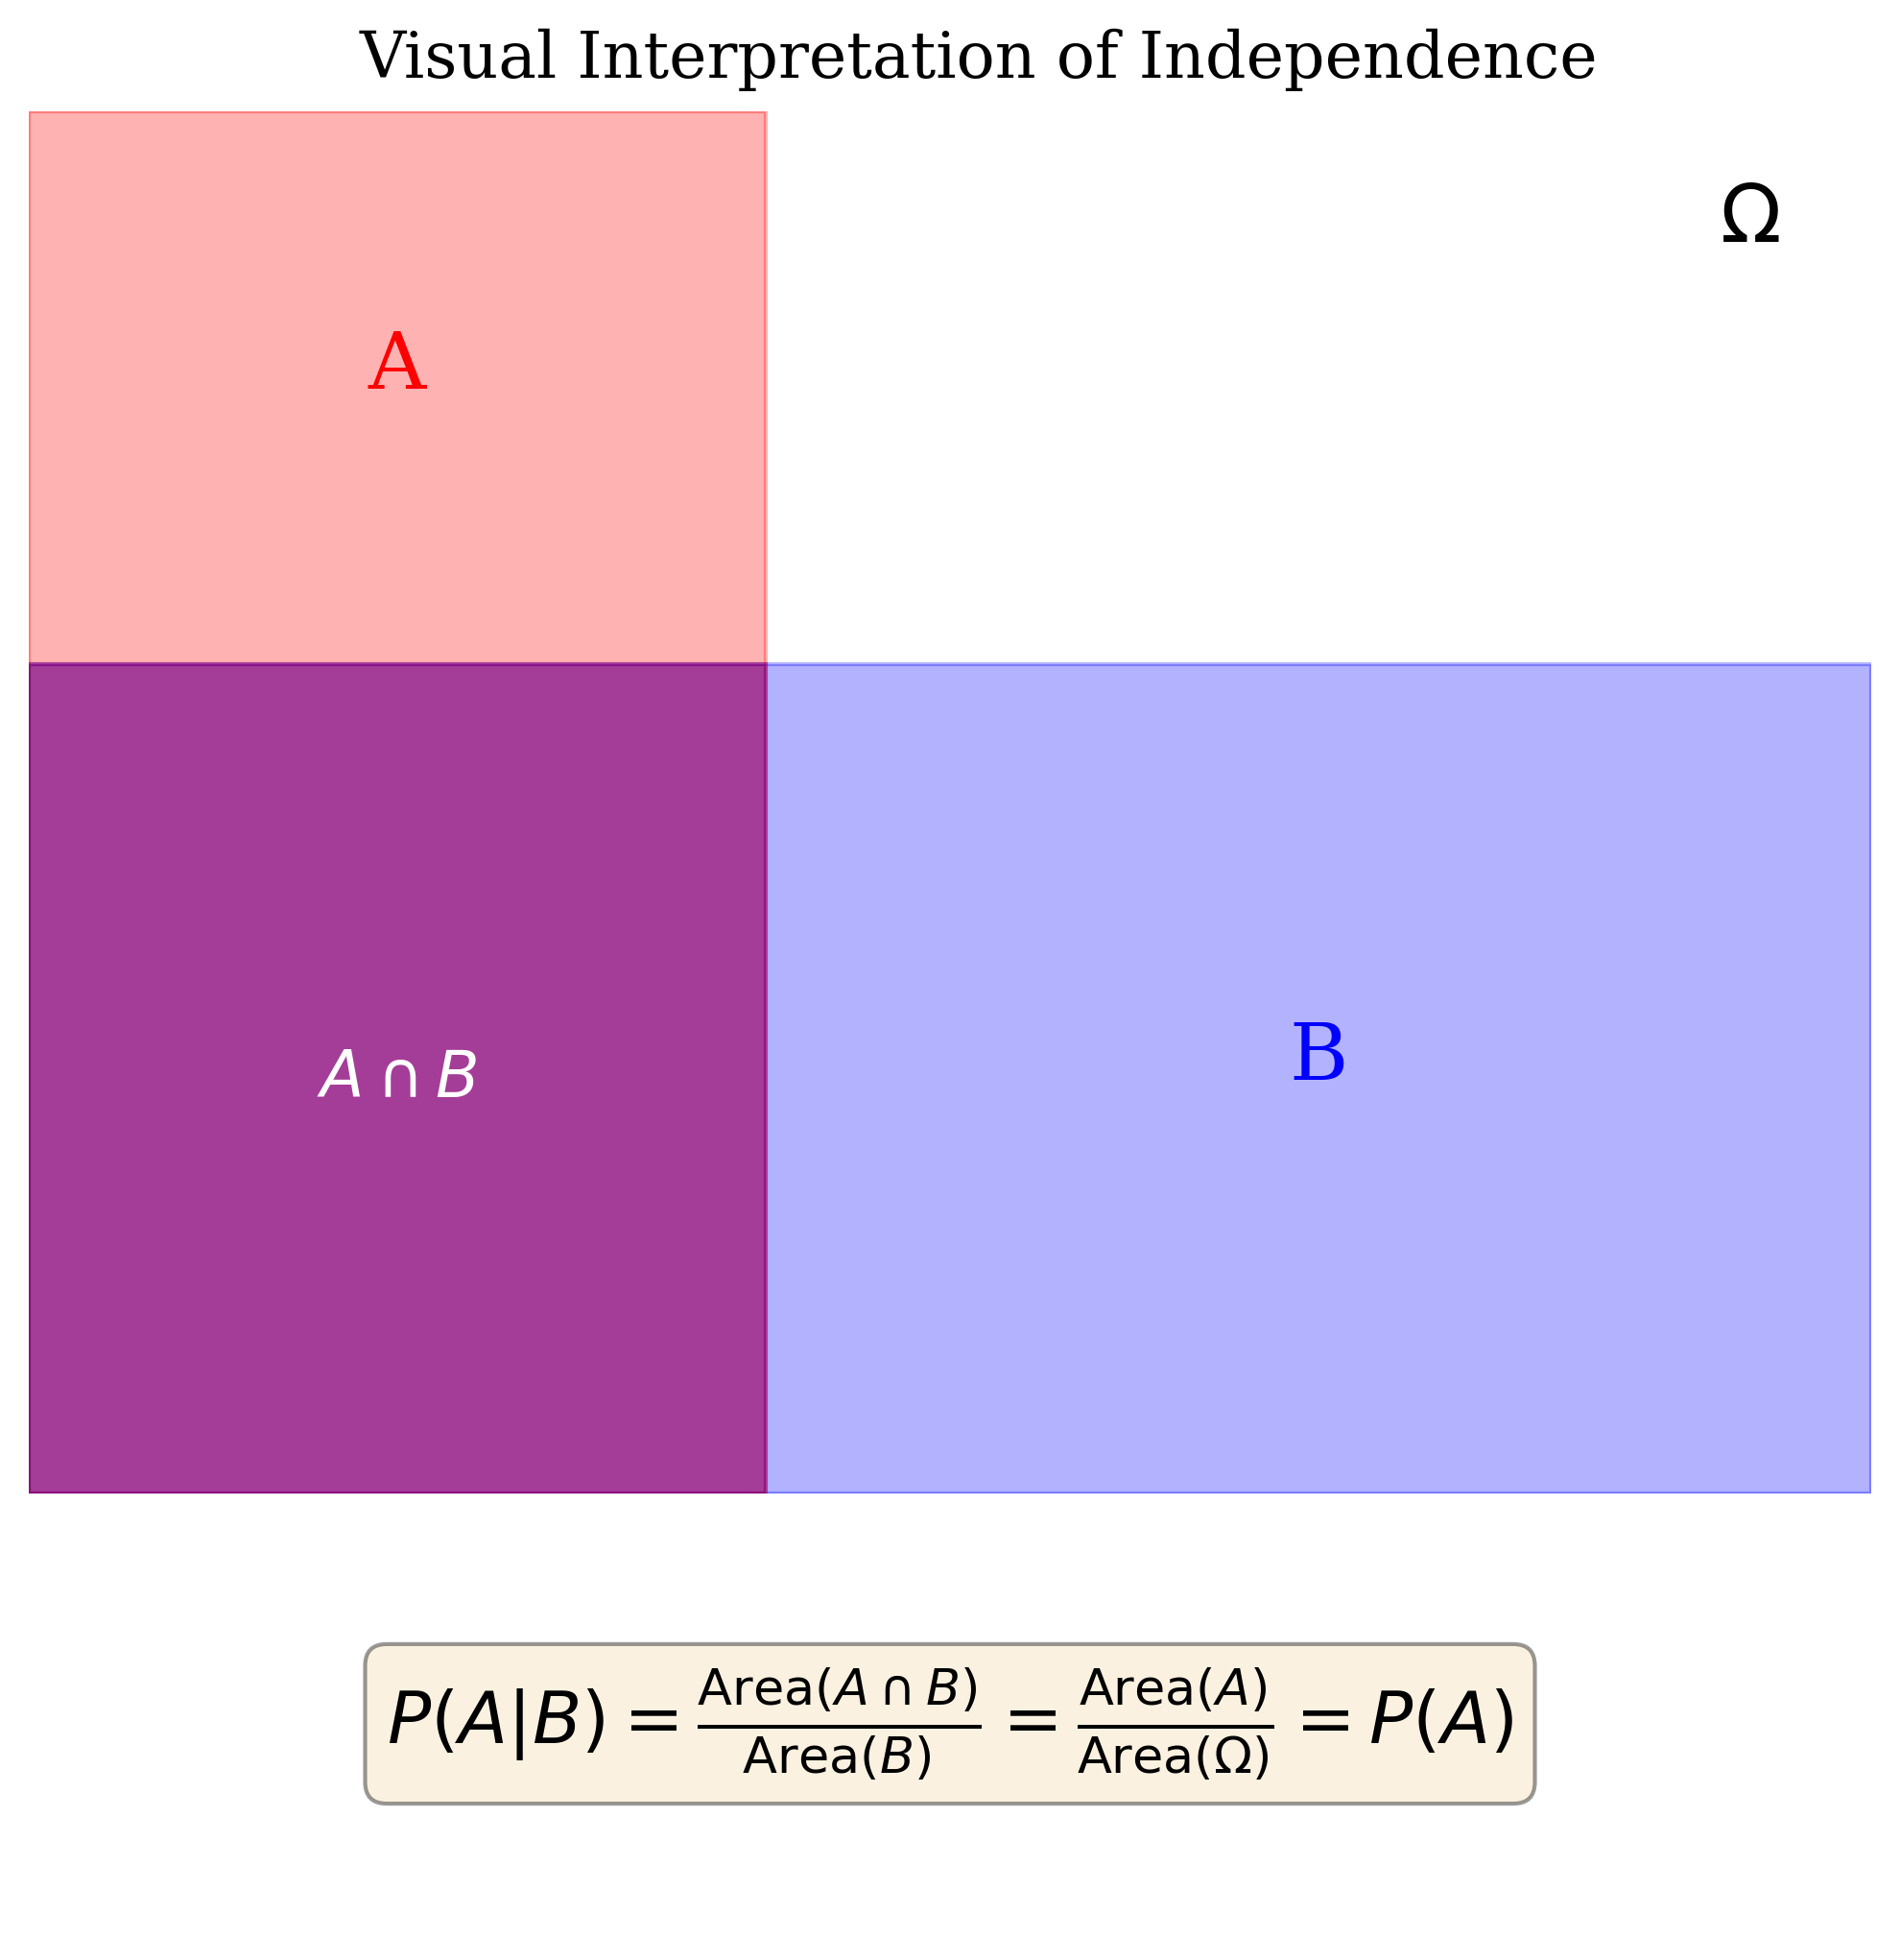
\includegraphics[width=0.7\textwidth]{figure_3.png}
    \caption{Visual interpretation of Independence: $\condProb{A}{B} = \Prob{A}$ \cite{Chan}.}
    \label{fig:indep_vis}
\end{figure}

\subsection{Distinction: Independent vs. Disjoint}
It is crucial to differentiate between independent events and disjoint (mutually exclusive) events \cite{Chan}. These concepts are fundamentally different.
\begin{itemize}
    \item \textbf{Disjoint:} Events cannot occur simultaneously ($A \intersect B = \emptySet$, thus $\Prob{A \intersect B} = 0$).
    \item \textbf{Independent:} Occurrence of one event does not alter the probability of the other ($\Prob{A \intersect B} = \Prob{A}\Prob{B}$).
\end{itemize}
If $\Prob{A}>0$ and $\Prob{B}>0$, disjoint events are necessarily \textbf{dependent}. Knowing A occurred implies B did not occur ($\condProb{B}{A} = 0$, which is generally not equal to $\Prob{B}$) \cite{Chan}.

\begin{figure}[ht]
    \centering
    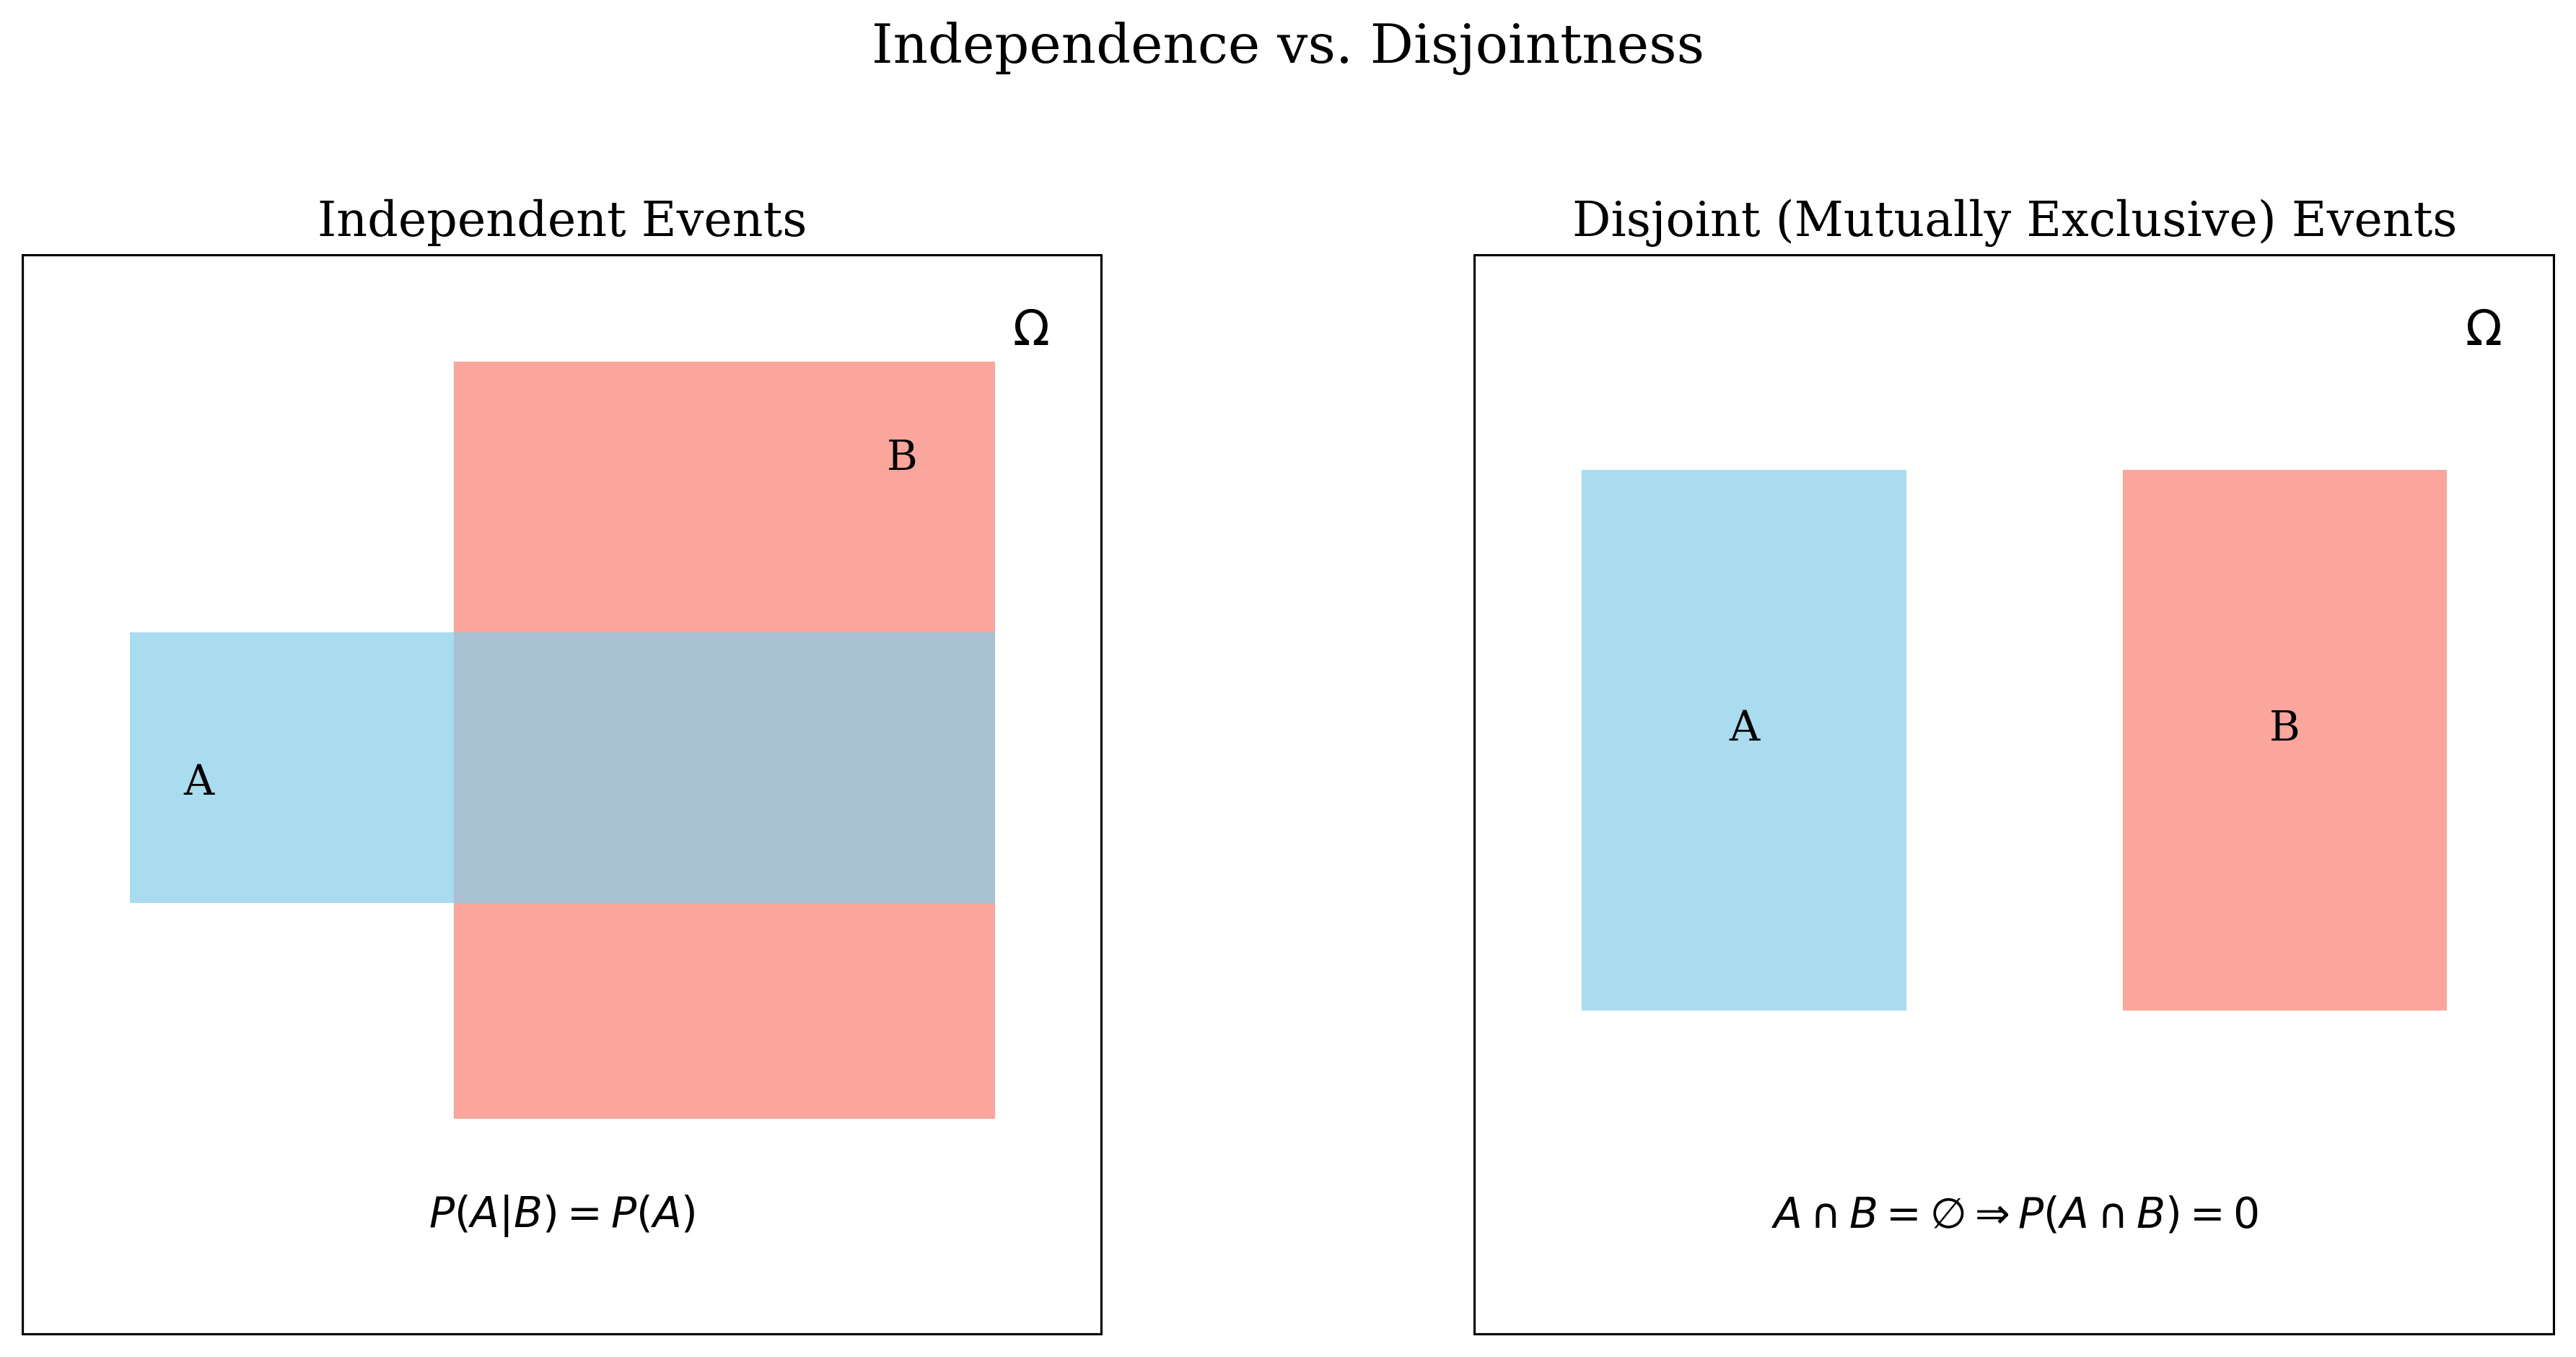
\includegraphics[width=0.9\textwidth]{figure_4.png}
    \caption{Comparing Independence ($\condProb{A}{B}=\Prob{A}$) and Disjointness ($A \intersect B = \emptySet$) \cite{Chan}.}
    \label{fig:indep_disjoint}
\end{figure}

\subsection{Properties of Independence}
A key property is that if events A and B are independent, then their complements are also independent in any combination \cite{FacultyNotes}.

\begin{theorem}[Independence of Complements \cite{FacultyNotes}]
\textbf{(Theorem)} If A and B are independent events, then the following pairs are also independent:
\begin{enumerate}
    \item $\comp{A}$ and B
    \item A and $\comp{B}$
    \item $\comp{A}$ and $\comp{B}$
\end{enumerate}
\end{theorem}
\begin{proof}[Proof (that A and $\comp{B}$ are independent)]
\textbf{(Proof)} Event A can be partitioned into two disjoint sets: $A = (A \intersect B) \union (A \intersect \comp{B})$ \cite{FacultyNotes}.
By Axiom III: $\Prob{A} = \Prob{A \intersect B} + \Prob{A \intersect \comp{B}}$.
Since A and B are independent, $\Prob{A \intersect B} = \Prob{A}\Prob{B}$.
Substituting: $\Prob{A} = \Prob{A}\Prob{B} + \Prob{A \intersect \comp{B}}$.
Rearranging: $\Prob{A \intersect \comp{B}} = \Prob{A} - \Prob{A}\Prob{B} = \Prob{A}(1 - \Prob{B})$.
Since $1 - \Prob{B} = \Prob{\comp{B}}$, we have $\Prob{A \intersect \comp{B}} = \Prob{A}\Prob{\comp{B}}$. By Definition 3.1, A and $\comp{B}$ are independent. (Proven). The other cases follow similar logic \cite{FacultyNotes}.
\end{proof}

\subsection{Examples of Independence}

\begin{example}[Die Roll \cite{Chan, Ross}]
\textbf{(Example)}
\begin{itemize}
    \item Experiment: Roll two fair six-sided dice. Sample space has 36 equally likely outcomes.
    \item Let $A = \{\text{first die is 3}\}$. Then $\Prob{A} = 6/36 = 1/6$.
    \item Let $B = \{\text{sum is 7}\}$. $B = \{(1,6), (2,5), (3,4), (4,3), (5,2), (6,1)\}$. $\Prob{B} = 6/36 = 1/6$.
    \item The intersection is $A \intersect B = \{(3,4)\}$. $\Prob{A \intersect B} = 1/36$.
\end{itemize}
\textbf{Check Independence:} We compare $\Prob{A \intersect B}$ with $\Prob{A}\Prob{B}$.
\[ \Prob{A}\Prob{B} = (1/6)(1/6) = 1/36 \]
Since $\Prob{A \intersect B} = \Prob{A}\Prob{B}$, events A and B are \textbf{independent} \cite{Chan, Ross}.
\end{example}

\begin{example}[Die Roll (Dependent) \cite{Ross, Chan}]
\textbf{(Example)}
\begin{itemize}
    \item Same experiment as above.
    \item Let $A = \{\text{first die is 3}\}$. $\Prob{A} = 1/6$.
    \item Let $B = \{\text{sum is 8}\}$. $B = \{(2,6), (3,5), (4,4), (5,3), (6,2)\}$. $\Prob{B} = 5/36$.
    \item The intersection is $A \intersect B = \{(3,5)\}$. $\Prob{A \intersect B} = 1/36$.
\end{itemize}
\textbf{Check Independence:} We compare $\Prob{A \intersect B}$ with $\Prob{A}\Prob{B}$.
\[ \Prob{A}\Prob{B} = (1/6)(5/36) = 5/216 \]
Since $\Prob{A \intersect B} \neq \Prob{A}\Prob{B}$ ($1/36 \neq 5/216$), events A and B are \textbf{dependent} \cite{Chan}. Intuitively, knowing the first die is 3 increases the chance the sum is 8 compared to the baseline probability of the sum being 8.
\end{example}

\subsection{Independence of Multiple Events}
The concept extends naturally to collections of more than two events.

\begin{definition}[Independence of n Events \cite{FacultyNotes, Ross}]
\textbf{(Definition)} A collection of events $E_1, E_2, \dots, E_n$ is said to be \textbf{mutually independent} (or simply \textbf{independent}) if, for \textit{every} subcollection of $k$ events $\{E_{i_1}, E_{i_2}, \dots, E_{i_k}\}$ (where $2 \le k \le n$):
\[ \Prob{E_{i_1} \intersect E_{i_2} \intersect \dots \intersect E_{i_k}} = \Prob{E_{i_1}}\Prob{E_{i_2}}\dots\Prob{E_{i_k}} \]
This condition must hold for all pairs, all triplets, ..., and for the intersection of all $n$ events \cite{Ross, FacultyNotes}.
\end{definition}

\begin{remark}[Pairwise vs. Mutual Independence \cite{Ross, Chan}]
\textbf{(Remark)} It is important to note that events can be \textbf{pairwise independent} (meaning $\Prob{E_i \intersect E_j} = \Prob{E_i}\Prob{E_j}$ for all $i \neq j$) without being mutually independent (the product rule fails for some triplet or larger subset). Mutual independence requires the product rule to apply to all possible subsets \cite{Ross, Chan}.
\end{remark}

\begin{example}[Pairwise vs. Mutual Independence \cite{Ross}]
\textbf{(Example)}
\begin{itemize}
    \item An urn contains 4 balls labeled 1, 2, 3, 4. One ball is drawn randomly.
    \item Define events: $E = \{1, 2\}$, $F = \{1, 3\}$, $G = \{1, 4\}$.
    \item $\Prob{E} = \Prob{F} = \Prob{G} = 2/4 = 1/2$.
\end{itemize}
\textbf{Pairwise Independence Checks:}
\begin{itemize}
    \item $\Prob{E \intersect F} = \Prob{\{1\}} = 1/4$. $\Prob{E}\Prob{F} = (1/2)(1/2) = 1/4$. They are equal.
    \item $\Prob{E \intersect G} = \Prob{\{1\}} = 1/4$. $\Prob{E}\Prob{G} = (1/2)(1/2) = 1/4$. They are equal.
    \item $\Prob{F \intersect G} = \Prob{\{1\}} = 1/4$. $\Prob{F}\Prob{G} = (1/2)(1/2) = 1/4$. They are equal.
\end{itemize}
Thus, E, F, and G are pairwise independent \cite{Ross}.
\textbf{Mutual Independence Check:}
\begin{itemize}
    \item $\Prob{E \intersect F \intersect G} = \Prob{\{1\}} = 1/4$.
    \item $\Prob{E}\Prob{F}\Prob{G} = (1/2)(1/2)(1/2) = 1/8$.
\end{itemize}
Since $\Prob{E \intersect F \intersect G} \neq \Prob{E}\Prob{F}\Prob{G}$, the events E, F, G are pairwise independent but \textbf{not mutually independent} \cite{Ross}.
\end{example}

\section{Law of Total Probability}

This law provides a method to calculate the probability of an event B by conditioning on a partition of the sample space \cite{FacultyNotes}. It decomposes the calculation of $\Prob{B}$ into simpler conditional probabilities.

\begin{definition}[Partition \cite{FacultyNotes}]
\textbf{(Definition)} A collection of events $\{A_1, A_2, \dots, A_n\}$ is a \textbf{partition} of the sample space $\samplespace$ if:
\begin{enumerate}
    \item The events are mutually exclusive (disjoint): $A_i \intersect A_j = \emptySet$ for all $i \neq j$.
    \item The union of the events covers the entire sample space: $\bigcup_{i=1}^{n} A_i = \samplespace$.
\end{enumerate}
Essentially, exactly one of the events $A_i$ must occur \cite{Ross}.
\end{definition}

\begin{theorem}[Law of Total Probability \cite{Ross, Chan, FacultyNotes}]
\textbf{(Theorem)} Let $\{A_1, A_2, \dots, A_n\}$ be a partition of the sample space $\samplespace$, such that $\Prob{A_i} > 0$ for all $i$. Then for any event B:
\[ \Prob{B} = \sum_{i=1}^{n} \Prob{B \intersect A_i} = \sum_{i=1}^{n} \condProb{B}{A_i}\Prob{A_i} \]
\end{theorem}
\begin{proof}
\textbf{(Proof)} Since $\{A_1, \dots, A_n\}$ is a partition of $\samplespace$, the sets $\{B \intersect A_1, \dots, B \intersect A_n\}$ form a partition of event B. That is, $B = \bigcup_{i=1}^{n} (B \intersect A_i)$, and these intersection events $(B \intersect A_i)$ are mutually exclusive because the $A_i$ are mutually exclusive \cite{FacultyNotes, Chan}.
By Axiom III of probability (additivity for disjoint events):
\[ \Prob{B} = \Prob{\bigcup_{i=1}^{n} (B \intersect A_i)} = \sum_{i=1}^{n} \Prob{B \intersect A_i} \]
Applying the multiplication rule $\Prob{B \intersect A_i} = \condProb{B}{A_i}\Prob{A_i}$ (since $\Prob{A_i} > 0$) to each term yields the result:
\[ \Prob{B} = \sum_{i=1}^{n} \condProb{B}{A_i}\Prob{A_i} \]
(Proven) \cite{FacultyNotes, Chan, Ross}.
\end{proof}

\begin{remark}
\textbf{(Remark)} The Law of Total Probability states that $\Prob{B}$ is a weighted average of the conditional probabilities $\condProb{B}{A_i}$, where the weights are the probabilities $\Prob{A_i}$ of the events in the partition \cite{Ross, Chan}. It allows computing $\Prob{B}$ by first conditioning on which of the mutually exclusive and exhaustive events $A_i$ occurs \cite{Ross}.
\end{remark}

\begin{figure}[ht]
    \centering
    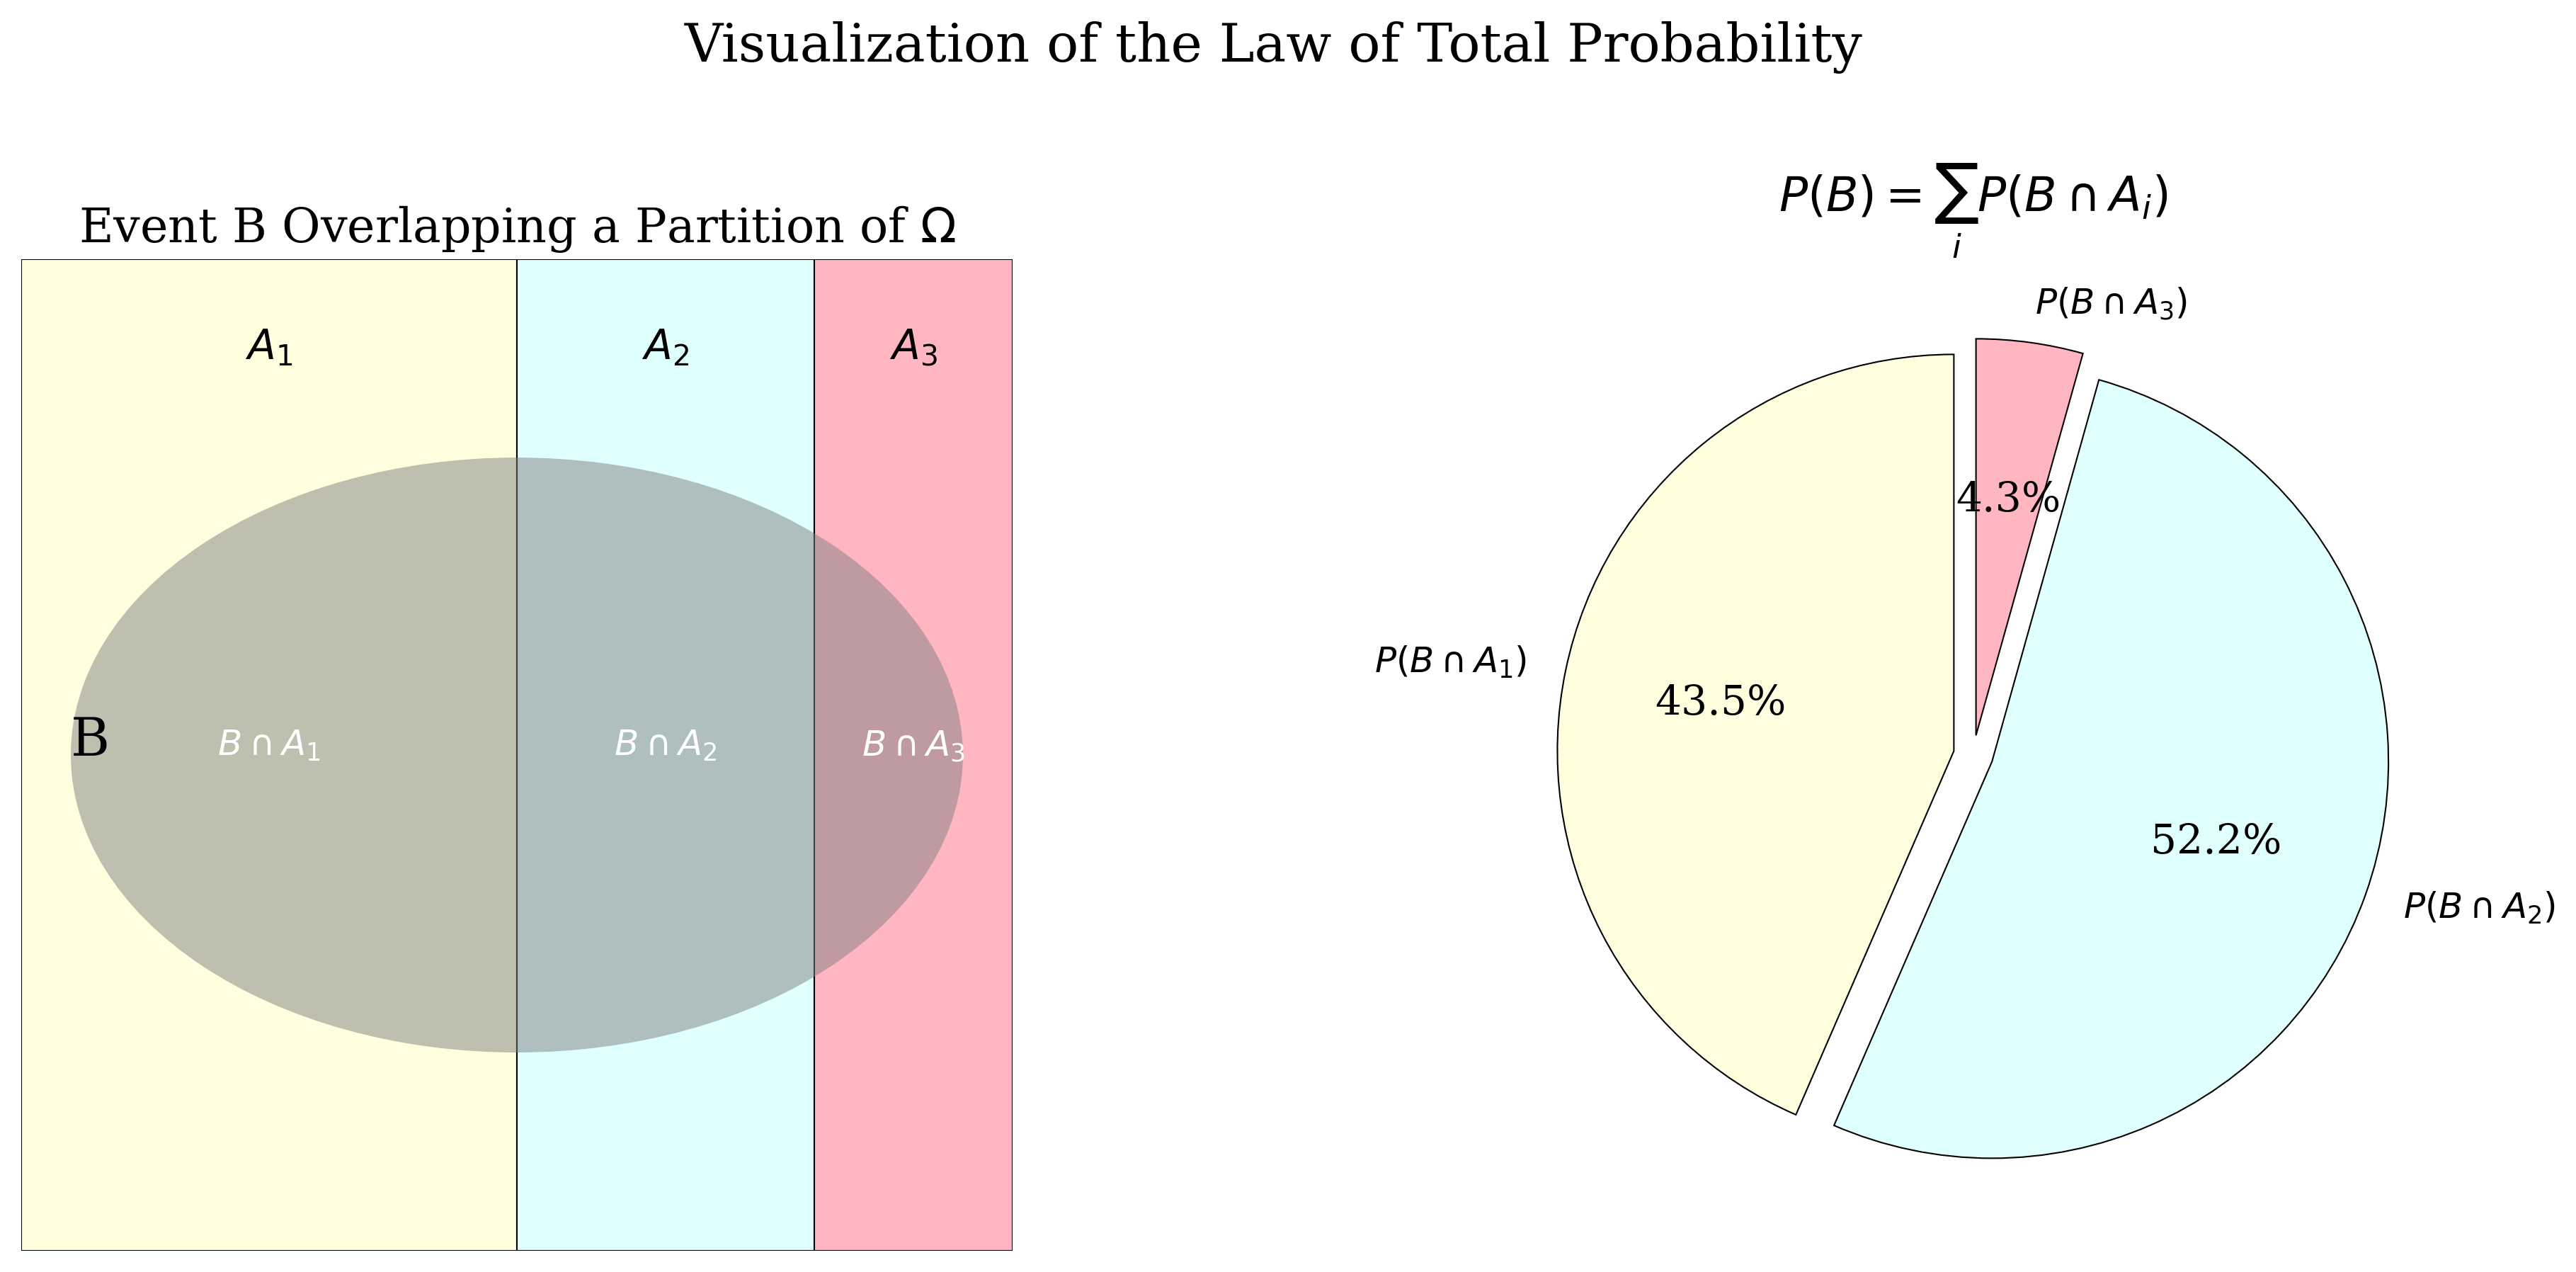
\includegraphics[width=0.9\textwidth]{figure_5.png}
    \caption{Visualization of the Law of Total Probability \cite{Chan, FacultyNotes}.}
    \label{fig:total_prob}
\end{figure}

\section{Bayes' Theorem}
Bayes' Theorem relates the conditional probability of an event A given B to the conditional probability of B given A. It is fundamental for statistical inference and updating beliefs based on evidence \cite{Chan}.

\begin{theorem}[Bayes' Theorem \cite{Ross, Chan, FacultyNotes}]
\textbf{(Theorem)} Let A and B be events with $\Prob{A}>0$ and $\Prob{B}>0$. Then:
\[ \condProb{A}{B} = \frac{\condProb{B}{A}\Prob{A}}{\Prob{B}} \]
\end{theorem}
\begin{proof}
\textbf{(Proof)} The theorem follows directly from the definition of conditional probability and the commutative property of intersection \cite{Chan, FacultyNotes}.
From the multiplication rule, we have two expressions for the joint probability $\Prob{A \intersect B}$:
\begin{enumerate}
    \item $\Prob{A \intersect B} = \condProb{A}{B}\Prob{B}$
    \item $\Prob{A \intersect B} = \Prob{B \intersect A} = \condProb{B}{A}\Prob{A}$
\end{enumerate}
Equating the right-hand sides gives:
\[ \condProb{A}{B}\Prob{B} = \condProb{B}{A}\Prob{A} \]
Dividing by $\Prob{B}$ (which is non-zero by assumption) yields Bayes' Theorem. (Proven).
\end{proof}

\subsection{Bayes' Formula with Total Probability}
Often, the denominator $\Prob{B}$ in Bayes' Theorem is not directly known. If we have a partition $\{A_1, \dots, A_n\}$ of the sample space, we can compute $\Prob{B}$ using the Law of Total Probability. Substituting this expansion into Bayes' Theorem gives the commonly used form:

\begin{corollary}[Full Bayes' Formula \cite{Ross, Chan, FacultyNotes}]
\textbf{(Corollary)} Let $\{A_1, \dots, A_n\}$ be a partition of $\samplespace$ with $\Prob{A_i} > 0$ for all $i$. Then for any event $A_j$ in the partition and any event B with $\Prob{B}>0$:
\[ \condProb{A_j}{B} = \frac{\condProb{B}{A_j}\Prob{A_j}}{\sum_{i=1}^{n} \condProb{B}{A_i}\Prob{A_i}} \]
This formula allows us to calculate the posterior probability $\condProb{A_j}{B}$ using the prior probabilities $\Prob{A_i}$ and the likelihoods $\condProb{B}{A_i}$ \cite{Ross, Chan}.
\end{corollary}

\begin{remark}[Terminology \cite{Chan}]
In the context of Bayes' Theorem $\condProb{A}{B} = \frac{\condProb{B}{A}\Prob{A}}{\Prob{B}}$:
\begin{itemize}
    \item $\Prob{A}$ is often called the \textbf{prior probability} of A (belief before observing B).
    \item $\condProb{A}{B}$ is the \textbf{posterior probability} of A (updated belief after observing B).
    \item $\condProb{B}{A}$ is the \textbf{likelihood} of observing B given A occurred.
    \item $\Prob{B}$ is the \textbf{evidence} or marginal probability of B.
\end{itemize}
\end{remark}

\section{Advanced Application: The Three Prisoners Problem}

\begin{example}[The Three Prisoners Problem \cite{Chan, Ross}]
\textbf{(Example)} This problem illustrates potential pitfalls in intuitive reasoning about conditional probability.
\begin{itemize}
    \item \textbf{Setup:} Prisoners A, B, C. One chosen randomly (prob 1/3 each) to be sentenced, the other two pardoned. Prisoner A asks a guard, who knows the outcome, to name one of the \textit{other} prisoners (B or C) who will be pardoned. The guard complies (if A is to be sentenced, the guard randomly chooses between B and C to name; if B is sentenced, guard names C; if C is sentenced, guard names B). Suppose the guard names B \cite{Chan}.
    \item \textbf{A's (Flawed) Reasoning:} "Initially, $\Prob{\text{A sentenced}} = 1/3$. After the guard says B is pardoned, only A and C remain as possibilities for sentencing. My probability must now be $1/2$." \cite{Chan, Ross}.
    \item \textbf{Analysis:} Let $X_A, X_B, X_C$ be the events that A, B, C are sentenced, respectively ($\Prob{X_A}=\Prob{X_B}=\Prob{X_C}=1/3$). Let $G_B$ be the event the guard says B is pardoned. We want to compute $\condProb{X_A}{G_B}$.
    \item \textbf{Guard's Protocol (Likelihoods):} Based on the rules the guard follows:
        \begin{itemize}
            \item $\condProb{G_B}{X_A} = 1/2$: If A is sentenced, B and C are pardoned; guard chooses one randomly \cite{Chan}.
            \item $\condProb{G_B}{X_B} = 0$: If B is sentenced, guard cannot name B \cite{Chan}.
            \item $\condProb{G_B}{X_C} = 1$: If C is sentenced, A and B are pardoned; guard must name B \cite{Chan}.
        \end{itemize}
    \item \textbf{Evidence $\Prob{G_B}$ (using Law of Total Probability):}
        \begin{align*} \Prob{G_B} &= \condProb{G_B}{X_A}\Prob{X_A} + \condProb{G_B}{X_B}\Prob{X_B} + \condProb{G_B}{X_C}\Prob{X_C} \\ &= (1/2)(1/3) + (0)(1/3) + (1)(1/3) = 1/6 + 0 + 1/3 = 1/2 \quad \cite{Chan}\end{align*}
    \item \textbf{Posterior Probability $\condProb{X_A}{G_B}$ (using Bayes' Theorem):}
        \[ \condProb{X_A}{G_B} = \frac{\condProb{G_B}{X_A}\Prob{X_A}}{\Prob{G_B}} = \frac{(1/2)(1/3)}{1/2} = 1/3 \quad \cite{Chan} \]
\end{itemize}
\textbf{Conclusion:} Prisoner A's probability of being sentenced remains $1/3$, unchanged by the guard's statement. The guard's statement $G_B$ provides no information about A's fate because the events $X_A$ and $G_B$ are independent in this scenario. A's intuitive reasoning was flawed because it didn't correctly account for the conditional nature of the guard's statement \cite{Chan, Ross}.
\end{example}

\section{Random Variable (Brief Definition)}

\begin{definition}[Random Variable \cite{FacultyNotes}]
\textbf{(Definition)} A \textbf{Random Variable} (RV), typically denoted by a capital letter (e.g., $X$), is a function that maps outcomes $\omega$ from a sample space $\samplespace$ to real numbers ($\reals$) \cite{FacultyNotes}.
\[ X: \samplespace \rightarrow \reals \]
It is a way to assign a numerical value to the result of a random experiment.
\end{definition}

\begin{figure}[ht]
    \centering
    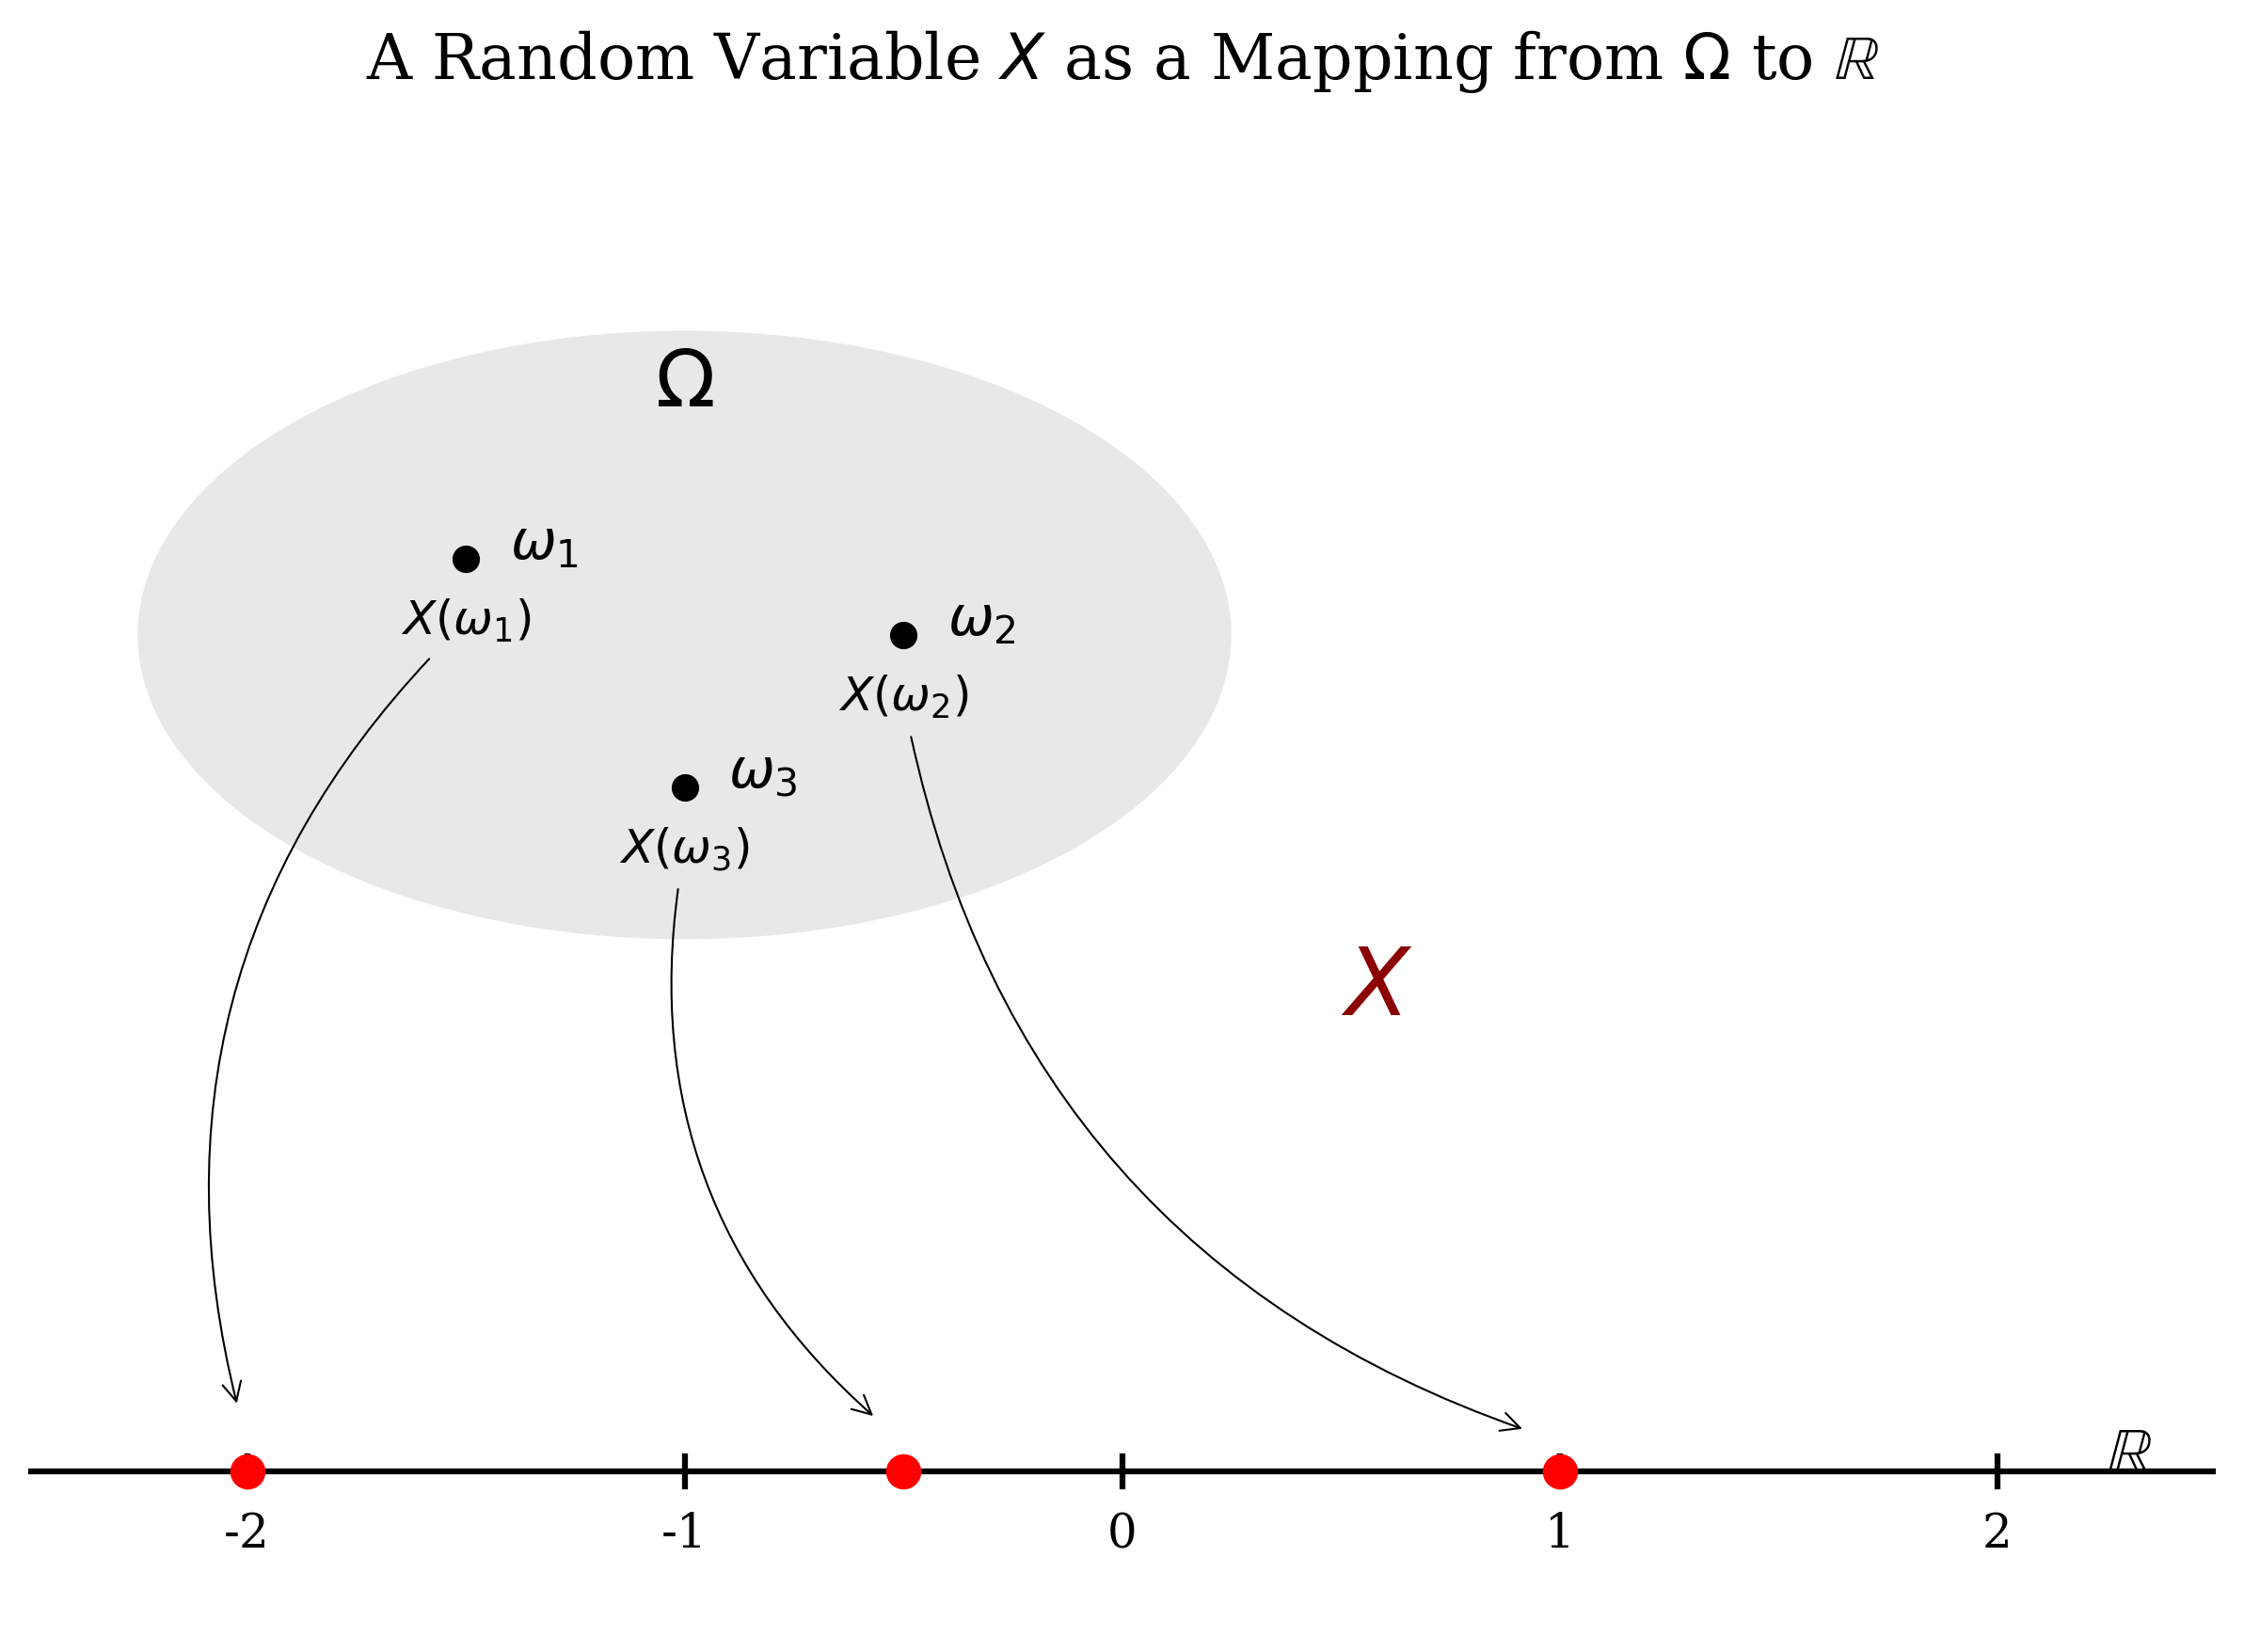
\includegraphics[width=0.9\textwidth]{figure_6.png}
    \caption{Visualization of a Random Variable as a function mapping outcomes to real numbers \cite{FacultyNotes}.}
    \label{fig:rv_vis}
\end{figure}

\newpage
\printbibliography

\end{document}